%%%% AAAI-27 anonymous submission -- SHORE-RL
%%%% Style files: aaai2027.sty / aaai2027.bst (official AAAI-27 author kit, v2027/05/04)
%%%% Build:  pdflatex main ; bibtex main ; pdflatex main ; pdflatex main
%%%% Main empirical claim: sustained final-window performance on
%%%% temporally extended manipulation tasks.

\documentclass[letterpaper]{article} % DO NOT CHANGE THIS
\usepackage[submission]{aaai2027}  % anonymous submission version
% aaai2027.sty loads the required newtxtext, helvet, and courier fonts.
\usepackage[hyphens]{url}  % DO NOT CHANGE THIS
\usepackage{graphicx} % DO NOT CHANGE THIS
\urlstyle{rm} % DO NOT CHANGE THIS
\def\UrlFont{\rm}  % DO NOT CHANGE THIS
\usepackage{natbib}  % DO NOT CHANGE THIS AND DO NOT ADD ANY OPTIONS TO IT
\usepackage{caption} % DO NOT CHANGE THIS AND DO NOT ADD ANY OPTIONS TO IT
\frenchspacing  % DO NOT CHANGE THIS
\setlength{\pdfpagewidth}{8.5in} % DO NOT CHANGE THIS
\setlength{\pdfpageheight}{11in} % DO NOT CHANGE THIS

\usepackage{amsmath}
\usepackage{amssymb}
\usepackage{booktabs}
\usepackage{multirow}
\usepackage{placeins}

\pdfinfo{
/TemplateVersion (2027.1)
}

\setcounter{secnumdepth}{2}

% ---- float placement: let more floats land near their text ----
\setcounter{topnumber}{3}
\setcounter{totalnumber}{4}
\renewcommand{\topfraction}{0.9}
\renewcommand{\textfraction}{0.05}
\renewcommand{\floatpagefraction}{0.7}

\newcounter{algorithm}

\title{SHORE-RL: Stable Long-Horizon Reinforcement Learning of Imitation
Policies via Temporal Localization}

\author{Anonymous Submission}
\affiliations{}

\begin{document}

\maketitle

\begin{abstract}
Imitation policies provide strong priors for robotic manipulation, yet their
performance is limited by demonstration coverage. Reinforcement learning (RL)
can improve a frozen imitation policy through a compact action residual, but
we find that several representative finetuning methods do not sustain their
early gains on temporally extended, sparse-feedback tasks. We introduce
\textbf{SHORE-RL}, which localizes residual learning in time along two
complementary paths. A navigator predicts a nearby latent waypoint from frozen
base-policy features, giving the residual actor a local decision context; an
independent progress reward supplies the critic with shorter-delay feedback.
The physical episode is unchanged, and the critic backs up the full shaped
return rather than terminating at the waypoint. The navigator is learned from
demonstrations without object poses or geometric goal distances, and the
reward can use either task stages or a
potential learned from the same offline data. On four long-horizon
DexMimicGen tasks, SHORE-RL maintains strong final-window success while
action-residual, noise-space, imitation-bootstrapped, and full-policy
finetuning baselines deteriorate below their frozen-policy references.
Controlled ablations show that waypoint conditioning, demonstration
anchoring, and progress feedback interact in a task-dependent manner, with
the complete method performing most consistently. SHORE-RL also improves a
frozen $\pi_0$ policy on two LIBERO tasks. Finally, residual training in
learned-dynamics imagination improves a frozen VLA on three real-robot tasks,
providing initial evidence that temporal localization extends beyond direct
simulator interaction.
\end{abstract}

% =====================================================================
\section{Introduction}
% =====================================================================
Imitation policies---from behavior-cloned controllers to
vision-language-action (VLA) models---provide powerful priors for robotic
manipulation, but inherit the errors and coverage limits of their
demonstrations~\cite{ross2011dagger,mandlekar2021matters}. Reinforcement
learning (RL) offers a route beyond this ceiling. In particular, residual RL
keeps the pretrained policy fixed and learns only a bounded action
correction~\cite{johannink2019residual}, preserving the imitation prior while
reducing the dimension of online adaptation. Recent frozen-policy methods
demonstrate the sample efficiency of this strategy~\cite{resfit2025residual}.
Constraining \emph{where} adaptation occurs, however, does not resolve
\emph{when} its consequences become observable: each local correction is
still optimized through a task-level return that may depend on many subsequent
decisions.

This temporal issue becomes visible in the learning dynamics. In our
cross-task diagnostic (Fig.~\ref{fig:vanilla-collapse}), vanilla residual RL
remains stable on a group of shorter or less compositionally demanding tasks,
but deteriorates after transient improvements on four multi-stage tasks.
Because these groups differ in more than horizon, the comparison establishes
an empirical association rather than a controlled causal effect. It
nevertheless exposes a practical failure mode: under sparse, delayed
feedback~\cite{arjona2019rudder,harutyunyan2019hindsight,hung2019optimizing,andrychowicz2017hindsight},
the critic receives weak evidence about individual corrections, and residual
drift can compound across a sequence. We therefore ask: \emph{can residual
finetuning be stabilized by making both action selection and learning
feedback more temporally local?}

\begin{figure}[t]
\centering
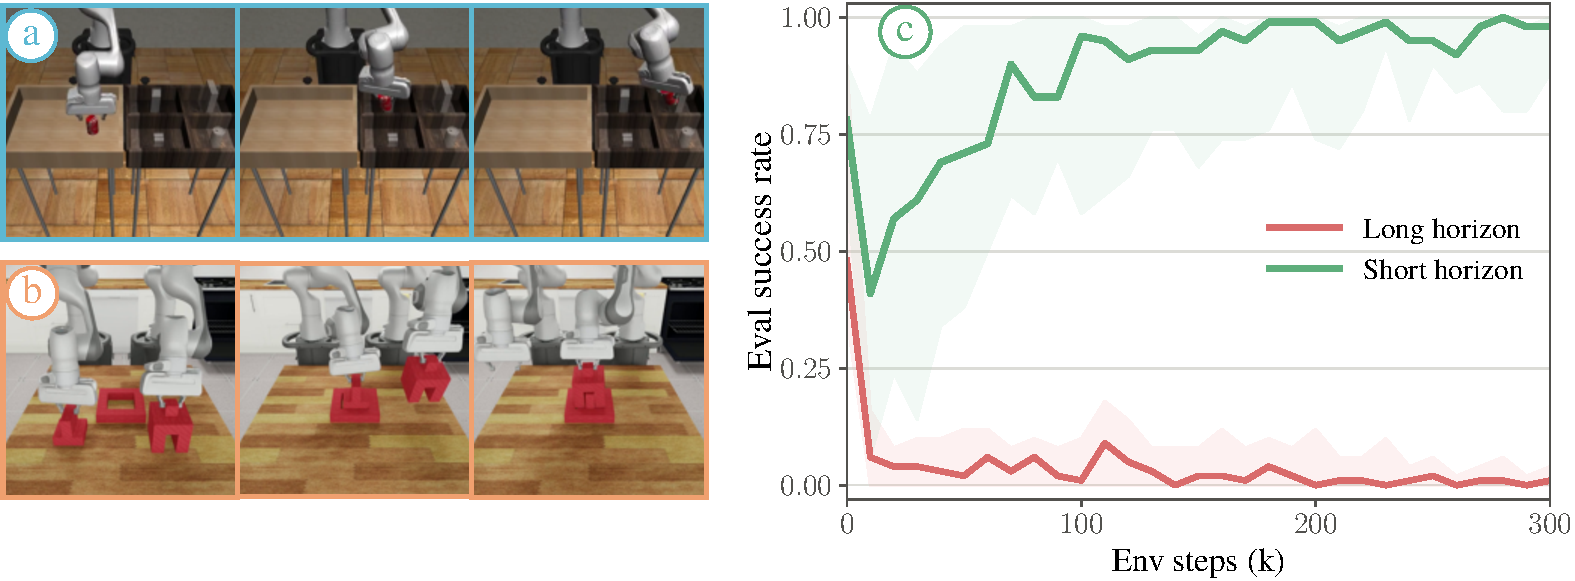
\includegraphics[width=\columnwidth]{figure/fig_vanilla_collapse.pdf}
\caption{\textbf{Cross-task diagnostic of vanilla residual RL.} (a,b)
Representative RoboMimicGen \textsc{Can} (short-horizon) and
DexMimicGen \textsc{PieceAssembly} (long-horizon) tasks. (c) Median with
min--max band across four short-horizon tasks---RoboMimicGen \textsc{Can} and \textsc{Square},
and DexMimicGen \textsc{CanSort} and \textsc{Box Clean Up} (green)---and four
long-horizon DexMimicGen tasks---\textsc{PieceAssembly}, \textsc{Pouring}, \textsc{LiftTray}, and \textsc{Threading}
(red). The task groups also differ in composition and reward structure; the
plot motivates temporal localization but does not isolate horizon as a causal
variable.}
\label{fig:vanilla-collapse}
\end{figure}

We introduce \textbf{SHORE-RL}, a temporally localized framework for adapting a
frozen imitation policy. The method separates two roles that are often
conflated. On the actor path, a navigator learned from demonstrations supplies
a nearby latent waypoint, localizing the context for each residual correction.
On the critic path, an independent progress signal makes useful feedback
available at a transition or stage boundary. The waypoint is neither a
terminal state nor the source of the shaping reward, and the critic continues
to optimize the global return. Consequently, SHORE-RL does not shorten the
physical episode or the Bellman backup; it reduces the \emph{effective
decision-conditioning} and \emph{feedback} horizons.

The navigator operates on frozen base-policy features and requires neither
object poses nor geometric goal distances. For critic feedback, we study both
a hand-specified stage bonus and policy-invariant potential shaping learned
from demonstrations. We evaluate sustained, rather than peak, improvement
using final-window success and full learning curves. We also study a
learned-dynamics extension in which the same residual objective is optimized
in imagined rollouts before physical evaluation. Our contributions are:

\begin{figure*}[t]
\centering
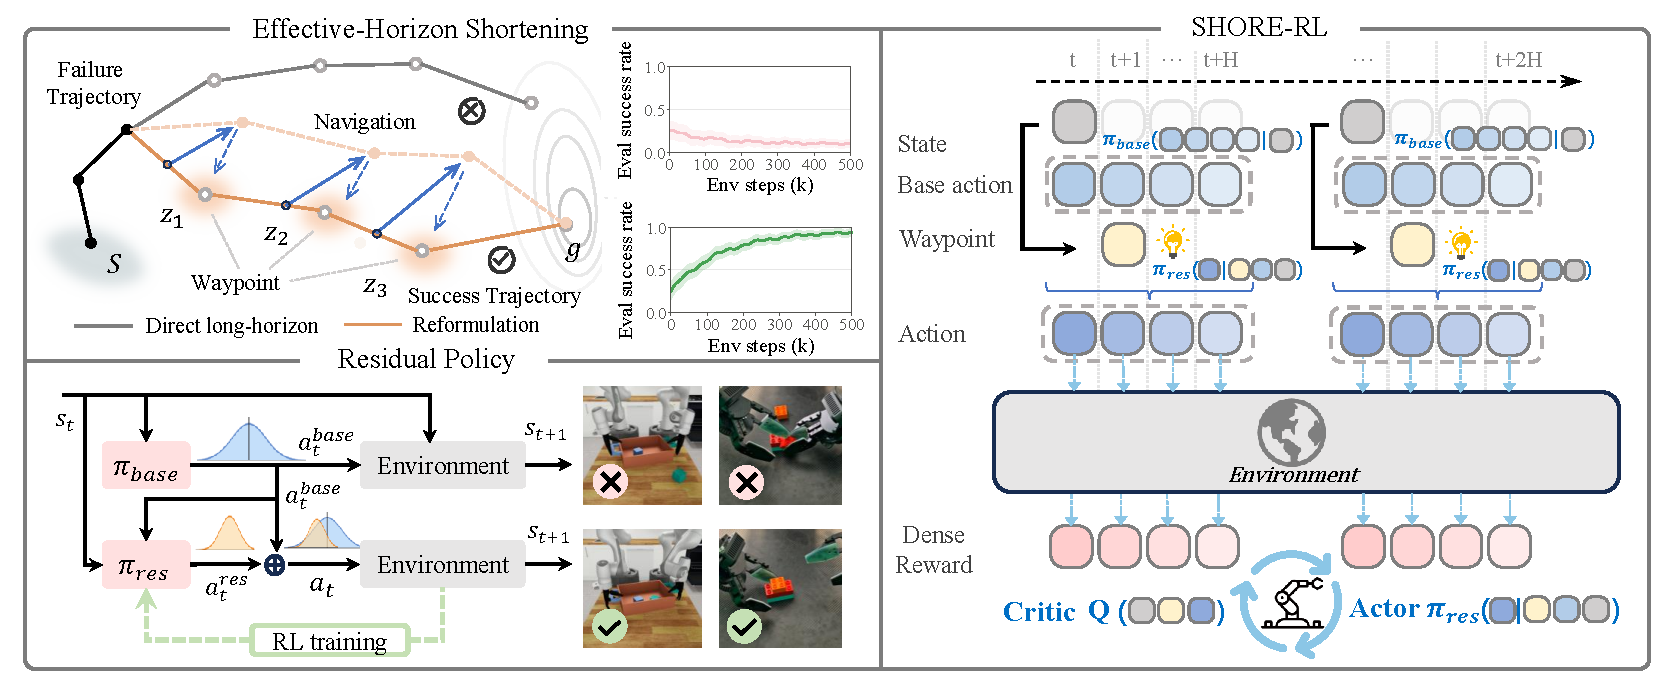
\includegraphics[width=\textwidth]{figure/framework.pdf}
\caption{\textbf{Overview of SHORE-RL.}
\emph{Upper left:} Direct goal conditioning leaves each correction tied to a
distant outcome, whereas latent waypoints provide local decision context.
\emph{Lower left:} In the overall residual-RL framework, the frozen base policy
and the trainable residual policy jointly produce the executed action, and
environment transitions are used for residual-policy training. \emph{Right:}
SHORE-RL instantiates this framework over successive action chunks. A navigator
predicts a latent waypoint that conditions the residual actor, while an
independent dense progress reward trains the TD3 critic without consuming or
evaluating the waypoint. Neither path changes the physical task horizon.}
\label{fig:framework}
\end{figure*}
\begin{itemize}
\item We formulate temporal localization for frozen-policy RL and instantiate
it with two explicitly separated mechanisms: a demonstration-derived latent
waypoint for residual action selection and an independent progress signal for
critic learning.
\item We develop a bounded, waypoint-conditioned residual learner that
preserves the pretrained policy and uses only demonstrations and frozen
features for local goal context. We additionally provide a learned-potential
alternative to task-specific stage shaping.
\item Across four long-horizon DexMimicGen tasks, two LIBERO tasks, ACT and
$\pi_0$ base policies, and three real-robot tasks trained in learned-dynamics
imagination, we evaluate sustained performance against four finetuning
families and analyze the interactions among waypoints, behavior anchoring,
and reward feedback.
\end{itemize}

% =====================================================================
\section{Related Work}
\label{sec:related}
% =====================================================================
\paragraph{RL Finetuning of Imitation Policies.}
Behavior cloning provides a strong initialization for robot control but remains limited
by demonstration quality and coverage~\cite{ross2011dagger,mandlekar2021matters}. Online RL can improve this initialization, and
prior-data methods improve sample efficiency by leveraging demonstrations or offline
experience during online learning~\cite{ball2023efficient,nakamoto2023calql,zhang2023pex,li2023explore,rajeswaran2018learning,nair2018overcoming,pertsch2021accelerating}. IBRL retains the imitation policy as an
action proposal and uses learned values to choose between imitation and RL
actions~\cite{hu2023imitation}. These methods primarily address initialization, data
reuse, or how strongly the learned policy remains anchored to imitation. Our focus is
sustained final-window performance when temporal composition is extended.

\paragraph{Residual and Latent-Space Policy Adaptation.}
Residual RL freezes a controller and learns an additive action
correction~\cite{johannink2019residual,yuan2025policydecorator}. ResFit applies this parameterization to
behavior-cloned manipulation policies and combines it with sample-efficient off-policy
learning from prior data~\cite{resfit2025residual,ball2023efficient}. DSRL instead
optimizes the initial noise of a frozen diffusion or flow policy, moving adaptation
into a latent sampling space~\cite{wagenmaker2025dsrl}. These approaches differ in the
\emph{space} in which adaptation occurs and in how it is constrained around the base~\cite{ren2025dppo,wang2023diffusion}.
They do not provide each residual correction with a temporally local objective.

\paragraph{Temporal Abstraction and Progress Shaping.}
Temporal abstraction decomposes a long task into intermediate
goals~\cite{nachum2018hiro,fang2022ptp,shi2023skimo,zheng2024prise,sutton1999between,kulkarni2016hierarchical,dietterich2000maxq}. HIQL, for
example, learns a high-level latent subgoal together with a learned goal-conditioned
policy that reaches it~\cite{park2023hiql}. Existing RL-finetuning methods for
frozen imitation policies instead adapt actions, latent noise, or action
selection without a temporally local residual context. SHORE-RL conditions
only the frozen-base residual on a value-ranked near-future feature, without
introducing a separate low-level policy or terminating the return at the
waypoint. Progress shaping is complementary:
transition-level feedback may come from a stage bonus or from potential
differences~\cite{ng1999policy,devlin2012dynamic,wiewiora2003principled}.

\paragraph{World-Model Robot Learning as an Extension.}
Learned dynamics models provide policy-learning experience when direct robot
interaction is expensive~\cite{hafner2020dreamer,janner2019mbpo,hansen2024tdmpc2,mazzaglia2023choreographer,wu2023daydreamer}.
RISE uses an action-conditioned video model for robot policy
improvement~\cite{yang2026rise}. Video prediction can also provide an
action-free reward signal for RL~\cite{escontrela2023viper}. We similarly use learned
dynamics as a training environment, while retaining the same frozen-base
residual objective.

% =====================================================================
\section{Preliminaries}
% =====================================================================
\paragraph{Frozen-Base Residual Adaptation.}
We model each task as an episodic, partially observable manipulation problem
with latent state $s_t$, observation $o_t$, action $a_t$, task reward $r_t$, discount
$\gamma\in[0,1)$, and horizon $T$. The policy acts from observations, and
performance is measured by the expected discounted task return. We focus on
long-horizon settings with sparse or delayed task feedback. Given a frozen
imitation base policy $\pi_b$ and demonstration dataset $\mathcal D$, residual
adaptation~\cite{johannink2019residual,resfit2025residual} optimizes only the
residual-policy parameters $\theta$ while keeping $\pi_b$ fixed:
\begin{equation}
\begin{aligned}
a_t^b&=\pi_b(o_t),\quad \delta_t\in\Delta,\quad
a_t=\Pi_{\mathcal A}[a_t^b+\delta_t],\\
\theta^\star&\in\arg\max_\theta
\mathbb E\!\left[\sum_{t=0}^{T-1}\gamma^t r_t\right],
\qquad \pi_b\ \text{fixed}.
\end{aligned}
\label{eq:frozen-base-residual-adaptation}
\end{equation}
Here $\Delta$ is a bounded residual set, and $\Pi_{\mathcal A}$ projects the
combined action onto the valid action space. SHORE-RL retains this objective
and action interface while supplying each correction with more local context
and feedback.

\paragraph{Subgoal-Guided Policy Learning.}
A long-horizon goal can be decomposed into shorter goal-reaching segments,
allowing the policy to act toward intermediate subgoals rather than only the
final task outcome~\cite{sutton1999between,nachum2018hiro}. Expectile
regression can learn from offline data a value signal that ranks progress
toward a goal~\cite{kostrikov2022iql}. For action-free goal-conditioned
trajectories, the value conditions on the current state and a sampled
goal~\cite{park2023hiql}:
\begin{equation}
\mathcal L_V
=
\mathbb E\!\left[
\ell_2^\tau\!\left(
 r_g+\gamma m_g\bar V(s_{t+1},g)-V(s_t,g)
\right)\right],
\label{eq:goal-value-background}
\end{equation}
where $g$ is a sampled goal, $r_g$ is the goal-reaching reward, $m_g$ is its
continuation mask, $\ell_2^\tau$ is the expectile loss, and $\bar V$ is a
slow target. A high-level policy over demonstrated future states can then be
learned by advantage-weighted regression~\cite{peng2019awr,park2023hiql},
which assigns greater weight to future states with higher goal-conditioned
advantage and provides candidate subgoals for the downstream policy.

\paragraph{Potential-based reward shaping.}
For a fixed state potential $\Phi$, potential-based reward
shaping~\cite{ng1999policy} uses
\begin{equation}
 r_t^\Phi=r_t+\gamma\Phi(s_{t+1})-\Phi(s_t),
\label{eq:pbs-background}
\end{equation}
where $s_t$ is a generic state and $\Phi$ is held fixed during policy
optimization. Across a trajectory, the shaping terms telescope. With a zero
terminal potential, the shaped return differs from the original return only
by the policy-independent boundary term $-\Phi(s_0)$, so the set of optimal
policies is preserved.

% =====================================================================
\section{Method: SHORE-RL}
% =====================================================================
Figure~\ref{fig:framework} summarizes SHORE-RL: a frozen base policy proposes
the nominal action, a base-feature navigator supplies a latent waypoint to
the residual actor and critic, and a separate reward constructor supplies
dense critic feedback. Algorithm~\ref{alg:shore-unified} details the resulting
training loop. At each rollout decision, the frozen base action is combined
with a waypoint-conditioned residual, and the resulting transition is assigned
a shaped reward and stored in replay. SHORE-RL then samples demonstrations and
replay transitions to update the critic ensemble and, at delayed intervals,
the residual actor.

\subsection{Temporal Localization}
SHORE-RL leaves the MDP horizon $T$ unchanged and does not truncate the TD
target at a waypoint. Instead, it introduces two operational notions of
effective horizon. The \emph{decision-conditioning horizon} is localized by
training the navigator toward demonstrated future features sampled at most
$k$ steps ahead. This training window does not guarantee that a predicted
waypoint will be reached within $k$ physical steps at deployment. The
\emph{feedback horizon} is localized by issuing progress information at a
transition or stage boundary rather than only at task completion. The critic
still estimates the global shaped return. Accordingly, a waypoint is a local
control context, not a new terminal state, option boundary, or truncated
planning target.

\subsection{Waypoint-Conditioned Residual Policy}
\label{sec:hier}
Following Eq.~\eqref{eq:frozen-base-residual-adaptation}, at each residual-policy
decision $t$, the base policy proposes $a_t^b$, the navigator produces
$z_t$, and the residual actor samples
$\delta_t\sim\pi_{\mathrm{res}}(\cdot\mid o_t,a_t^b,z_t)$; the
environment executes the valid projection of $a_t^b+\delta_t$. Each critic
conditions on the current observation, waypoint, and stored combined action
rather than receiving $a_t^b$ separately. The actor and critics share a
trainable multi-view encoder distinct from the frozen base encoder and operate
on visual-proprioceptive observations. We train with
TD3~\cite{fujimoto2018addressing} and RLPD online--demonstration
mixing~\cite{ball2023efficient}.

Let $x_t=(o_t,a_t^b,z_t)$. For demonstrations, define
$x_t^D=(o_t^D,a_t^{b,D},z_t^D)$ and
$\delta_t^D=a_t^D-a_t^{b,D}$. With $K$ critics, the delayed actor update is
\begin{equation}
\begin{aligned}
\mathcal L_{\mathrm{res}}
={}&-\mathbb E_{\mathcal B_{\mathrm{mix}}}\!\left[
 \frac{1}{K}\sum_{i=1}^{K}
 Q_i\!\left(o_t,z_t,
 \Pi_{\mathcal A}[a_t^b+\mu_\theta(x_t)]\right)\right]\\
&+\lambda_{\mathrm{BC}}\,
\mathbb E_{\mathcal D}\!\left[
\left\|\mu_\theta(x_t^D)-\delta_t^D\right\|_2^2\right].
\end{aligned}
\label{eq:residual-actor-objective}
\end{equation}
Here $\mathcal B_{\mathrm{mix}}$ is the online--demonstration replay mixture
and $z_t^D$ is defined below. Critics use an $n$-step TD3 target with the
minimum of two randomly selected target heads; target smoothing and update
details are deferred to the supplement.

\subsection{Base-Policy-Derived Waypoint Navigator}
\label{sec:value}
We form the navigator state
$e_t=\operatorname{Std}([\psi_b(o_t);q_t])$ from the frozen
base-encoder feature and available proprioception. The task goal $g_\star$ is
represented by the medoid of terminal
demonstration features. We pretrain $V_{\mathrm{gc}}(e_t,g)$ from
demonstrations using the objective in
Eq.~\eqref{eq:goal-value-background}, with
$r_g=\mathbf 1[e_t=g]-1$ and $m_g=1-\mathbf 1[e_t=g]$. Reaching a sampled
goal therefore gives reward $0$ and stops bootstrapping, while every other
state receives $-1$. The implementation uses twin value heads and stabilized targets.

We then train the navigator $\pi_h$ by advantage-weighted regression toward a
demonstrated future-state bottleneck no more than $k$ steps ahead:
\begin{equation}
\begin{aligned}
z_t^D&=\phi(e_t,e_{w_t}),\qquad 0<w_t-t\leq k,\\
A_t^h&=V_{\mathrm{gc}}(e_{w_t},g)-V_{\mathrm{gc}}(e_t,g),\\
\mathcal L_h
&=-\mathbb E\!\left[
\min\!\left\{\exp(\beta A_t^h),M\right\}
\log\pi_h(z_t^D\mid e_t,g)\right].
\end{aligned}
\label{eq:navigator-awr}
\end{equation}
Demonstration replay uses $z_t^D$, whereas online rollouts use the navigator
mean $z_t=\mathbb E_{\pi_h(\cdot\mid e_t,g_\star)}[z]$. During residual
learning, $\phi$ remains frozen. In the dual-arm experiments, we jointly
finetune the value heads and $\pi_h$ on equally mixed online and demonstration
trajectories; the LIBERO experiments keep both modules fixed. This distinction
and the corresponding schedules are reported in the supplement.

\subsection{Progress Feedback for Critic Learning}
\label{sec:pot}
Sparse success feedback is densified in one of two ways:
\begin{equation}
\widetilde r_t
=r_t+
\begin{cases}
 b[G_{t+1}-G_t]_+, & \text{stage-based},\\
 \gamma(1-d_t)\Phi(e_{t+1})-\Phi(e_t),
 & \text{self-derived}.
\end{cases}
\label{eq:shore-dense-reward}
\end{equation}
Here $b>0$ scales the stage bonus, and $\Phi(e)=cV_{\mathrm p}(e)$ is the
self-derived potential, with $c>0$ rescaling the single-state progress value
$V_{\mathrm p}$. For the first form, $G_t$ is a latched stage
index, so the bonus is paid only when a new stage is completed; it is useful
when a predefined task decomposition is available, but carries no
policy-invariance claim. For the second, $d_t$ indicates a true terminal
transition. We train the
separate single-state progress value $V_{\mathrm p}$ on successful
demonstrations with an expectile-TD objective and freeze it before residual
learning. Thus the second line instantiates Eq.~\eqref{eq:pbs-background} for
the finite-horizon objective, with terminal bootstrapping masked. The navigator value
$V_{\mathrm{gc}}(e,g)$ selects actor waypoints, whereas $V_{\mathrm p}(e)$
constructs critic rewards; the networks are not shared. Both reward forms are
used only to construct critic targets. The stage bonus may change the optimal
policy; the potential-based alternative preserves the shaped objective's
policy ordering under the stated terminal convention.

\begin{figure}[!htbp]
\small
\refstepcounter{algorithm}\label{alg:shore-unified}
\setlength{\tabcolsep}{1.5pt}
\renewcommand{\arraystretch}{0.90}
\begin{tabular}{@{}r@{\,\,}p{0.83\columnwidth}@{}}
\toprule
\multicolumn{2}{@{}p{0.94\columnwidth}@{}}{\textbf{Algorithm \thealgorithm}\quad Unified SHORE-RL residual training}\\[1pt]
\multicolumn{2}{@{}p{0.94\columnwidth}@{}}{\hangindent=0.075\columnwidth\hangafter=1
\textbf{Require:}\hspace{0.35em}{\color{black!58}\itshape frozen base policy $\pi_b$, base feature extractor $\psi_b$, and waypoint bottleneck $\phi$; pretrained goal-conditioned value $V_{\mathrm{gc}}$ and navigator $\pi_h$; transition collector $\mathcal C$; environment-reward map $R$; shaping function $F$; replay sampler $\rho$; demonstration dataset $\mathcal D$; critic-update count $G$}}\\
\midrule
$1$ & Initialize zero-output residual actor $\mu_\theta$, critics $Q_{1:10}$, target networks, and replay $\mathcal B$ \\
$2$ & \textbf{for} each rollout decision $t$ \textbf{do} \\
$3$ & \quad Compute base action and navigator state:\newline
\makebox[\linewidth][c]{$a_t^b\gets\pi_b(o_t)$; $e_t\gets\operatorname{Std}([\psi_b(o_t);q_t])$} \\
$4$ & \quad Infer latent waypoint: $z_t\gets\mathbb E_{\pi_h(\cdot\mid e_t,g_\star)}[z]$ \\
$5$ & \quad Sample residual and project the combined action:\newline
\makebox[\linewidth][c]{$\delta_t\sim\pi_{\mathrm{res}}(\cdot\mid o_t,a_t^b,z_t)$; $a_t\gets\Pi_{\mathcal A}[a_t^b+\delta_t]$} \\
$6$ & \quad Execute or predict with $\mathcal C$:\newline
\makebox[\linewidth][c]{$(o_{t+1},r_t^{\mathrm{env}},d_t)\gets\mathcal C(o_t,a_t)$} \\
$7$ & \quad Shape reward: $\widetilde r_t\gets R(r_t^{\mathrm{env}})+F(o_t,o_{t+1},d_t)$ \\
$8$ & \quad Store $\tau_t=(o_t,z_t,a_t,\widetilde r_t,o_{t+1},d_t)$ in $\mathcal B$ \\
$9$ & \quad Optionally finetune $V_{\mathrm{gc}},\pi_h$ on mixed completed trajectories \\
$10$ & \quad \textbf{for} each critic update $g=1,\ldots,G$ \textbf{do} \\
$11$ & \quad\quad Sample mixed replay: $\mathcal B_g\sim\rho(\mathcal B,\mathcal D)$ \\
$12$ & \quad\quad Sample distinct $i,j\in\{1,\ldots,10\}$ uniformly:\newline
\makebox[\linewidth][c]{\hspace{2.8em}\scalebox{0.88}{$\displaystyle
\begin{aligned}
y_g\gets{}&\sum_{k=0}^{n-1}\gamma^k\widetilde r_{t+k}\\[-1pt]
 &+\gamma^n(1-d_{t:t+n})\min_{\ell\in\{i,j\}}\bar Q_\ell(o_{t+n},z_{t+n},a'_{t+n})
\end{aligned}$}}\newline
\hspace*{2em}Regress $Q_{1:10}$ toward $y_g$ \\
$13$ & \quad\quad \textbf{if} delayed actor update \textbf{then} \\
$14$ & \quad\quad\quad Update $\mu_\theta$ with Eq.~\eqref{eq:residual-actor-objective} \\
$15$ & \quad\quad \textbf{end if} \\
$16$ & \quad\quad Soft-update targets (actor only on delayed steps):\newline
\makebox[\linewidth][c]{$\bar\theta_Q\gets\tau\theta_Q+(1-\tau)\bar\theta_Q$}\newline
\makebox[\linewidth][c]{$\bar\theta_\mu\gets\tau\theta_\mu+(1-\tau)\bar\theta_\mu$} \\
$17$ & \quad \textbf{end for} \\
$18$ & \textbf{end for} \\
$19$ & \textbf{return} $\mu_\theta,\pi_h$ \\
\bottomrule
\end{tabular}
\end{figure}
\FloatBarrier

Here $d_{t:t+n}$ masks the bootstrap if a terminal transition occurs anywhere
in the $n$-step window, and $a'_{t+n}$ is the projected, target-smoothed
combined action. The exact target construction is given in the supplement.

Algorithm~\ref{alg:shore-unified} separates venue-specific collection from
the shared update. In simulation, $\mathcal C$ advances the task simulator,
$R$ supplies task reward, and $\rho$ draws equal online--demonstration
batches. For learned-dynamics training, $\mathcal C$ generates bounded rollouts
from recorded observations using a finetuned, frozen dynamics model. The
sampler $\rho$ then mixes recorded and imagined replay. The shaping function
$F$ can be either stage-based or self-derived in both simulation and
learned-dynamics training. The residual actor--critic update is shared across
settings; navigator finetuning is enabled only in the configurations identified
in the supplement. Exact venue configurations, action
mappings, and update schedules are given in the supplement.

\subsection{Residual Training with Learned Dynamics}
\label{sec:wm}
For the real-robot study, the collector $\mathcal C$ in
Algorithm~\ref{alg:shore-unified} generates short rollouts from a frozen
observation-prediction model $D$:
\begin{equation}
\begin{aligned}
&\widehat o_{t+1:t+H}=D(h_t,A_t),\\[2pt]
&\widetilde r_t^{\mathrm{imag}}
=r_t^{\mathrm{imag}}+\gamma\Phi(\widehat e_{t+1})-\Phi(e_t).
\end{aligned}
\label{eq:shore-imagination}
\end{equation}
Here $r_t^{\mathrm{imag}}$ is the task reward assigned to the imagined
transition. The model input $h_t$ is the fixed-length observation history,
$A_t$ is the combined action chunk, and $\widehat e_{t+1}$ is obtained by
re-encoding predicted multi-view frames with the frozen base encoder. Real
states seed short imagined rollouts, which are mixed with real replay while
limiting recursive prediction to control model error~\cite{janner2019mbpo,buckman2018steve}.
The dynamics model is used only during residual training, not at deployment.
No RL update is performed through physical robot interaction; hardware is
used for data collection and evaluation. Architecture, rollout, reward, and
buffer details are provided in the supplement.

% =====================================================================
\section{Experiments}
\label{sec:exp}
% =====================================================================

\subsection{Simulation Experiments}
\label{sec:exp-sim}

\begin{figure*}[t]
\centering
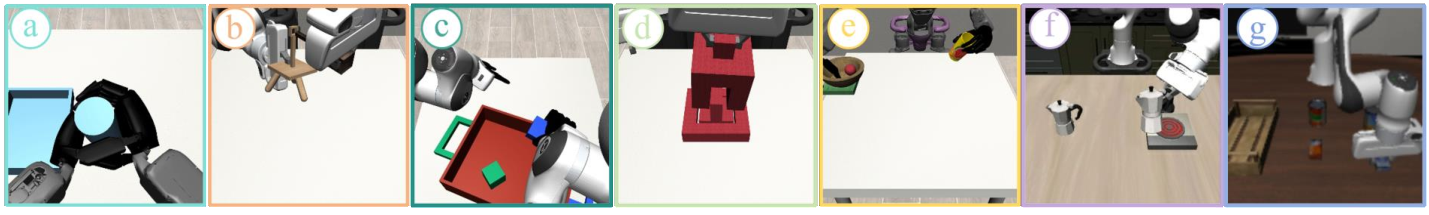
\includegraphics[width=\textwidth]{figure/sim_task.pdf}
\caption{\textbf{Simulated tasks.} The five DexMimicGen simulation tasks, left
to right: the shorter-horizon \textsc{CanSort} control followed by four
long-horizon dual-arm tasks, \textsc{Threading}, \textsc{LiftTray},
\textsc{PieceAssembly}, and \textsc{Pouring}. The two LIBERO tasks are
\emph{put both moka pots on the stove} (LIBERO-10 Task~8) and \emph{pick up
the cream cheese and put it in the tray} (LIBERO-90 Task~57).}
\label{fig:simtask}
\end{figure*}

\begin{figure*}[t]
\centering

\includegraphics[width=\textwidth]{\detokenize{figure/fig_long_horizon_anti_collapse_multiseed_curves copy.pdf}}
\caption{\textbf{Simulation results.} Evaluation success rate
versus environment steps on four long-horizon DexMimicGen tasks and the
shorter-horizon \textsc{CanSort} control. Lines are seed means with
$\pm 1$ s.e.m. bands.
SHORE-RL is compared with ResFit, DSRL, IBRL, and full-policy IQL. The thin
gray dotted reference in each panel marks the displayed SHORE-RL success at
zero environment steps, before residual learning. The displayed zero-step means for
\textsc{LiftTray}, \textsc{Threading}, and \textsc{CanSort} are $0.68$, $0.48$, and $0.90$,
respectively; the original zero-step s.e.m. widths are retained.}
\label{fig:main}
\end{figure*}

\paragraph{Tasks and Evaluation.}
We evaluate SHORE-RL on four long-horizon dual-arm dexterous manipulation tasks from
DexMimicGen~\cite{jia2024dexmimicgen}: \textsc{Threading},
\textsc{LiftTray}, \textsc{PieceAssembly}, and \textsc{Pouring}, plus the
shorter-horizon \textsc{CanSort} control (Fig.~\ref{fig:simtask}). The single-arm
extensions are LIBERO-10 \textsc{Task~8} (\emph{put both moka pots on the stove}) and
LIBERO-90 \textsc{Task~57} (\emph{pick up the cream cheese and put it in the tray})
\cite{liu2023libero} (Fig.~\ref{fig:libero}). We use ACT~\cite{zhao2023learning}
as the base policy for DexMimicGen and $\pi_0$~\cite{black2024pi0} for LIBERO.
DexMimicGen evaluations use $50$ episodes; LIBERO uses $10$ episodes, three seeds,
and $400$k environment steps. Our primary metric, \emph{final-window success}, is
computed by first averaging, for each seed, the evaluation checkpoints whose
environment-step counts lie in the final $20\%$ of the stated training budget
($400$k--$500$k for DexMimicGen and $320$k--$400$k for LIBERO, inclusive).
We then report the mean and s.e.m.\ across seeds. This metric deliberately
distinguishes sustained improvement from a transient peak; full learning
curves reveal any late-training deterioration.

\paragraph{Baselines.}
For the matched DexMimicGen comparison, we evaluate SHORE-RL against a frozen
BC reference and four RL-finetuning baselines with the same base-policy family,
offline demonstrations, interaction budget, number of seeds, and evaluation
schedule. This table compares complete methods; the component study below,
rather than the baseline table, isolates waypoint and reward design.
\emph{(i)~BC base}: the
frozen base policy with no RL, which determines whether adaptation sustains an
improvement. \emph{(ii)~ResFit}~\cite{resfit2025residual}: a frozen-base
action-residual method that uses equal sampling from offline demonstrations
and online replay.
\emph{(iii)~DSRL}~\cite{wagenmaker2025dsrl}: noise-space RL on the same base,
which tests whether changing the adaptation space prevents late degradation.
\emph{(iv)~IBRL}~\cite{hu2023imitation}: an off-policy method that uses a frozen
BC policy to propose alternative actions for both online action selection and
critic-target bootstrapping. \emph{(v)~IQL}: we instantiate
IQL~\cite{kostrikov2022iql} as a full-policy off-policy RL baseline that finetunes
the entire policy without retaining a frozen base, included as a non-residual control.

% =====================================================================
% PROVENANCE NOTES for Table 1.
% - IBRL cells use completed 500k-step matched-harness runs: 3 seeds per task.
% - DSRL and IQL cells are from completed 3-seed runs at 500k steps.
% =====================================================================
\begin{table}[t]
\centering
\small
\setlength{\tabcolsep}{0pt}
\begin{tabular*}{\columnwidth}{@{\extracolsep{\fill}}lcccc}
\toprule
Method & \textsc{Pouring} & \textsc{PieceAssembly} & \textsc{LiftTray} & \textsc{Threading} \\
\midrule
\textbf{SHORE-RL} & $\mathbf{0.91}_{\scriptscriptstyle\mathbf{\pm 0.02}}$ & $\mathbf{0.66}_{\scriptscriptstyle\mathbf{\pm 0.00}}$ & $\mathbf{0.85}_{\scriptscriptstyle\mathbf{\pm 0.01}}$ & $\mathbf{0.52}_{\scriptscriptstyle\mathbf{\pm 0.01}}$ \\
ResFit & $0.10_{\scriptscriptstyle\pm 0.07}$ & $0.02_{\scriptscriptstyle\pm 0.00}$ & $0.03_{\scriptscriptstyle\pm 0.01}$ & $0.01_{\scriptscriptstyle\pm 0.01}$ \\
DSRL & $0.26_{\scriptscriptstyle\pm 0.02}$ & $0.00_{\scriptscriptstyle\pm 0.00}$ & $0.00_{\scriptscriptstyle\pm 0.00}$ & $0.00_{\scriptscriptstyle\pm 0.00}$ \\
IBRL & $0.00_{\scriptscriptstyle\pm 0.00}$ & $0.10_{\scriptscriptstyle\pm 0.05}$ & $0.00_{\scriptscriptstyle\pm 0.00}$ & $0.00_{\scriptscriptstyle\pm 0.00}$ \\
IQL & $0.00_{\scriptscriptstyle\pm 0.00}$ & $0.00_{\scriptscriptstyle\pm 0.00}$ & $0.00_{\scriptscriptstyle\pm 0.00}$ & $0.40_{\scriptscriptstyle\pm 0.07}$ \\
\bottomrule
\end{tabular*}
\caption{Final-window success on the long-horizon simulation tasks. For each
method, we first average the per-seed evaluations from $400$k through $500$k
steps, inclusive (the final $20\%$ of the training budget), and report
mean$\pm$s.e.m.\ across seeds; each evaluation uses $50$ episodes. All methods
use three seeds, matched training budgets, and matched evaluation conditions.}
\label{tab:main}
\end{table}


% (world-model / real-robot deployment moved to the end of this section, after the sim
% results, so the SHORE-RL sim study reads as the main experiment.)

\paragraph{Sustained Long-Horizon Performance.}
Figure~\ref{fig:main} reports the complete learning trajectories, and
Table~\ref{tab:main} summarizes final-window success. SHORE-RL maintains high
success on \textsc{Pouring} and \textsc{LiftTray} and preserves substantial
gains on \textsc{PieceAssembly} and \textsc{Threading}. In the same
long-horizon tasks, ResFit, DSRL, IBRL, and full-policy IQL finish below their
respective frozen-policy references. The behavior of full-policy IQL indicates
that deterioration is not unique to an additive residual, while the
frozen-base baselines show that retaining an imitation anchor is not by itself
sufficient. ResFit remains near optimal on the \textsc{CanSort} control.
These results establish sustained gains for SHORE-RL in the tested tasks; they
do not, by themselves, isolate physical episode length from task composition,
reward density, or contact complexity.

\paragraph{Compatibility with ACT and \textbf{$\pi_0$.}}
Following the frozen-ACT experiments on DexMimicGen, we evaluate SHORE-RL with
a frozen $\pi_0$ VLA on LIBERO-10 \textsc{Task~8} and LIBERO-90
\textsc{Task~57}. Across both tasks, SHORE-RL reaches near-perfect final-window
success under the $400$k-step, three-seed protocol. The DSRL curves are
included as an indicative reference but were produced in a separate
query-20 harness, so they are not a strictly matched comparison. Together,
the ACT and $\pi_0$ experiments demonstrate compatibility with two tested
base-policy families (Fig.~\ref{fig:libero}); SHORE-RL still requires access
to frozen internal features and demonstration data and is therefore not a
black-box adapter.



\begin{figure}[t]
\centering
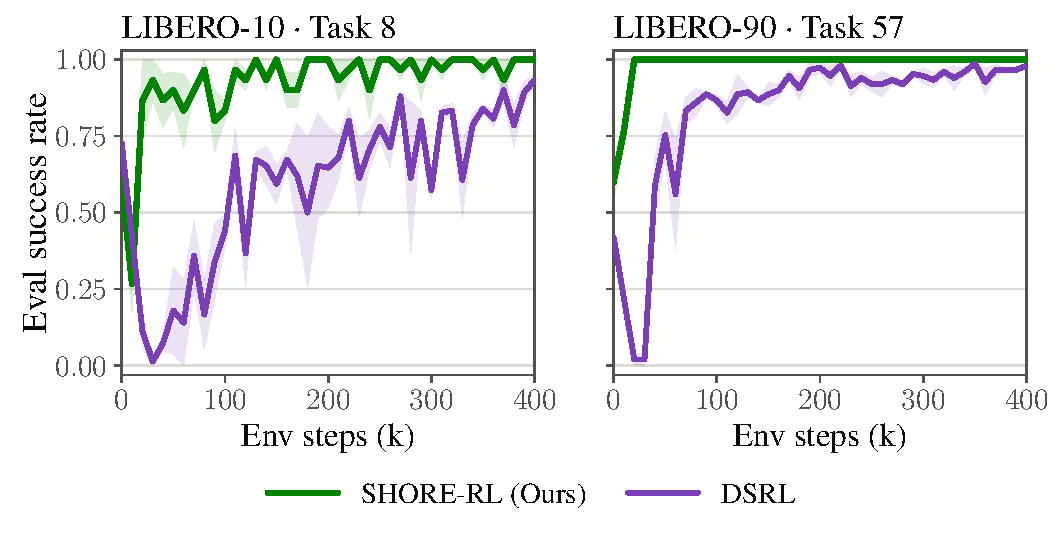
\includegraphics[width=\columnwidth]{figure/fig_libero10_aligned.pdf}
\caption{\textbf{LIBERO $\pi_0$ finetuning.}
Success on LIBERO-10 \textsc{Task~8} (left) and LIBERO-90 \textsc{Task~57}
(right) over $400$k steps. Curves are $3$-seed means with $\pm 1$ s.e.m.
SHORE-RL reaches near-perfect success on both tasks.}
\label{fig:libero}
\end{figure}

\subsection{Ablations}
\label{sec:exp-ablations}

\paragraph{Ablation Setup.}
We evaluate five matched configurations: the full SHORE-RL method and four
ablated variants, each removing one or more components---waypoint conditioning,
demo-BC, and stage shaping---as detailed in Table~\ref{tab:ablarms}.
All configurations use the same codebase, frozen features
$\psi$, offline data, action scale, evaluation protocol, and $400$k-step
training budget. The demo-BC coefficient is $0.1$ except in the configuration that
explicitly removes it. Figure~\ref{fig:ablbars} reports two long-horizon
tasks---\textsc{Pouring} and \textsc{PieceAssembly}---with
three seeds per configuration. For each seed, we average the evaluation success
rates over the final $20\%$ of training; bars report mean$\pm$s.e.\ across these
seed-level averages.

\begin{table}[t]
\centering\small\setlength{\tabcolsep}{4pt}
\resizebox{\columnwidth}{!}{%
\begin{tabular}{@{}lcccl@{}}
\toprule
Configuration & waypoint & BC & staged & removed \\
\midrule
\textbf{SHORE-RL}                       & on  & $0.1$ & on  & ---             \\
w/o stage shaping                       & on  & $0.1$ & off & shaping         \\
w/o waypoint                            & off & $0.1$ & on  & waypoint        \\
w/o waypoint \& stage shaping           & off & $0.1$ & off & waypoint $+$ staged \\
w/o demo-BC \& stage shaping            & on  & $0$   & off & BC $+$ staged   \\
\bottomrule
\end{tabular}
}
\caption{Matched component-ablation configurations with fixed action scale, evaluation
protocol, and comparison budget. SHORE-RL uses waypoint conditioning, demo-BC, and the
hand-designed per-stage bonus. The first three variants remove the listed
component or pair of components; the last keeps the waypoint while removing
both demo-BC and stage shaping.}
\label{tab:ablarms}
\end{table}

\paragraph{Component Ablations.}
Figure~\ref{fig:ablbars} summarizes matched component variants under a common
$400$k training budget on two long-horizon tasks. On
\textsc{PieceAssembly}, SHORE-RL reaches $0.65$, whereas every removal
variant reaches only $0.14$--$0.28$. Neither waypoint conditioning without
demo-BC and stage shaping ($0.23$) nor demo-BC with stage shaping but without
the waypoint ($0.28$) approaches the complete method. On \textsc{Pouring},
however, SHORE-RL ($0.93$) and the no-waypoint variant ($0.92$) are similar
within seed variation, while the remaining variants reach $0.73$--$0.80$.
Thus the experiment does not support a universal, additive waypoint gain.
Instead, it reveals task-dependent interactions: behavior anchoring and stage
feedback nearly compensate for the missing waypoint on \textsc{Pouring}, but
not on \textsc{PieceAssembly}. The full configuration is the only one that
performs strongly across both ablated tasks.

\begin{figure}[tbp]
\centering
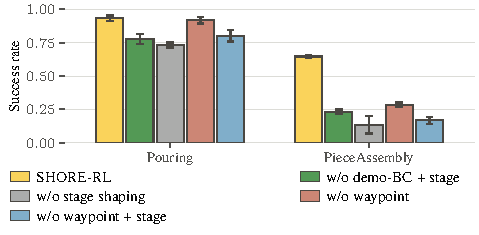
\includegraphics[width=0.85\columnwidth]{figure/fig_ablation_bars_400k.pdf}
\caption{\textbf{Ablation~A: matched component ablation.}
Success on two long-horizon dual-arm tasks with a common $400$k training
budget. Each per-seed score averages the evaluation success rates over the
final $20\%$ of training. Bars show means across three seeds, and error bars
show $\pm 1$ s.e.m.}
\label{fig:ablbars}
\end{figure}

\paragraph{Reward Form: Stage Bonus vs.\ Self-Derived Potential.}
\begin{figure}[!b]
\centering
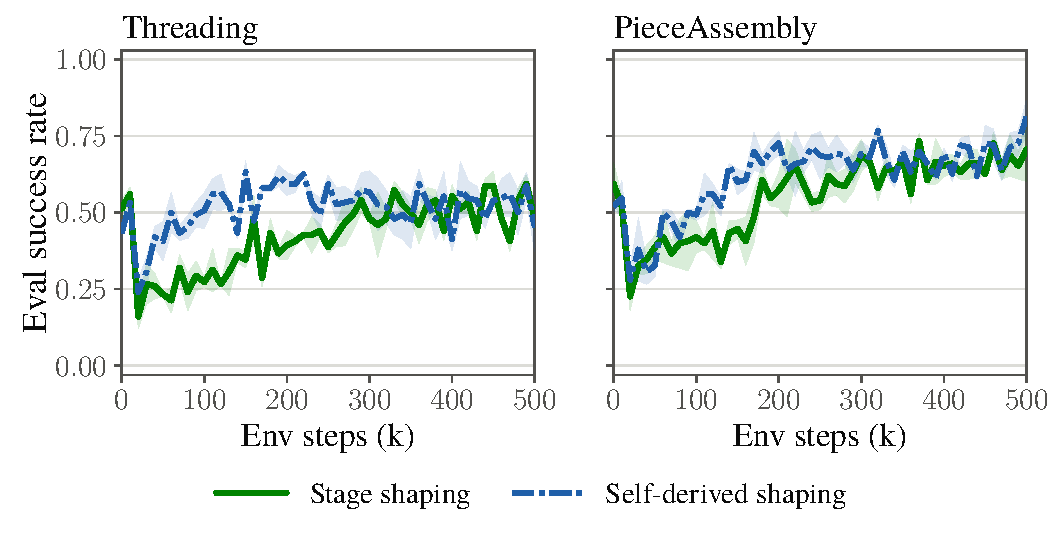
\includegraphics[width=\columnwidth]{figure/fig_staged_vs_pothiql_threading_piece_v2.pdf}
\caption{\textbf{Ablation~B: stage bonus vs.\ self-derived potential.}
Evaluation success versus environment steps on two stage-structured
long-horizon tasks. Both variants use waypoint conditioning, demo-BC, and online
joint finetuning; they differ only in the critic reward. \emph{Stage shaping}
uses the hand-designed per-stage bonus, whereas \emph{Self-derived shaping}
uses potential differences from $V_{\mathrm p}$. Lines are three-seed means
with $\pm 1$ s.e.m. bands.}
\label{fig:stagevspot}
\end{figure}


\begin{figure*}[!t]
\centering
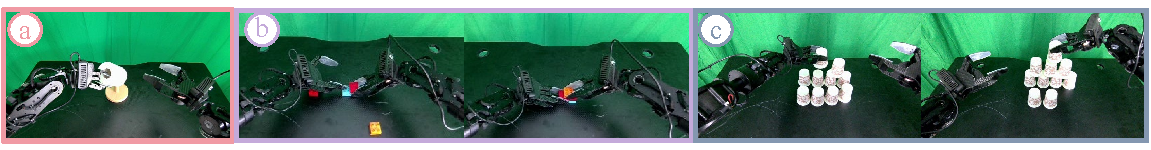
\includegraphics[width=\textwidth]{figure/real_task.pdf}
\caption{\textbf{Real-robot tasks.} Three bimanual tabletop tasks:
(a)~\textsc{Paper-Roll Placement}: picking up a paper roll and placing it
onto a holder; (b)~\textsc{Block Assembly}: assembling toy blocks; and
(c)~\textsc{Cup Stacking}: stacking paper cups into four levels.}
\label{fig:realtask}
\end{figure*}

\begin{figure*}[!t]
\centering
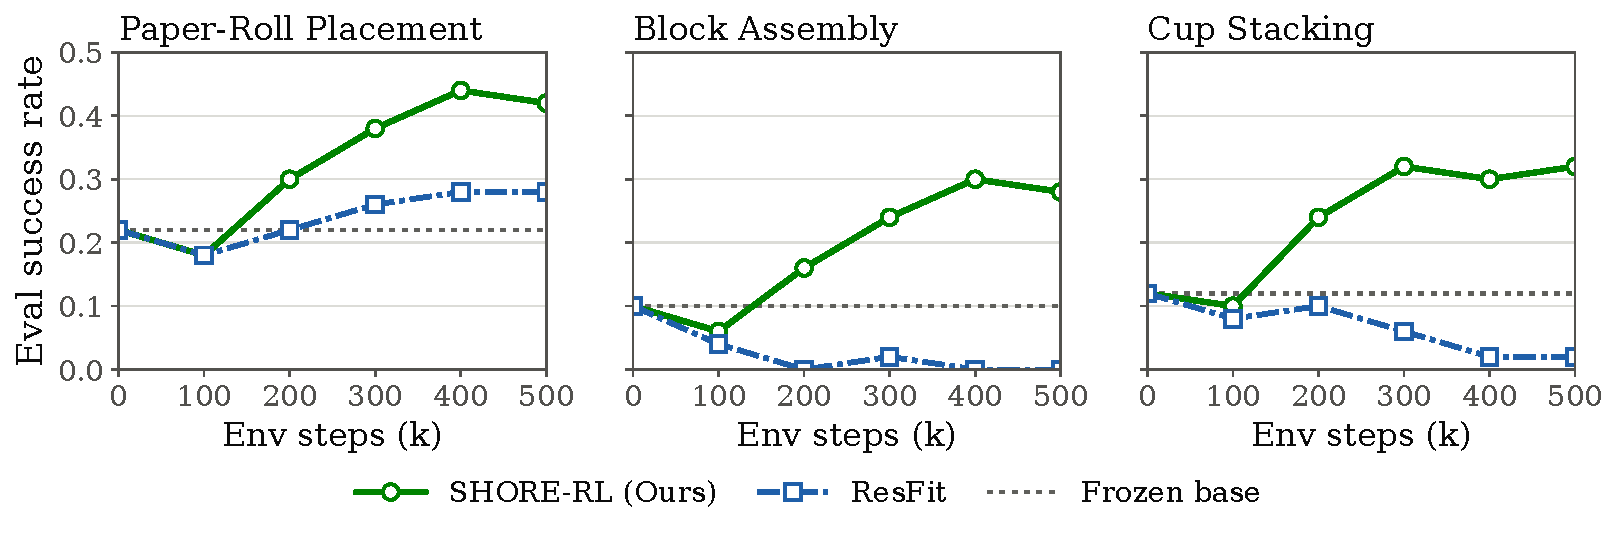
\includegraphics[width=0.65\textwidth]{figure/fig_real_robot_curves.pdf}
\caption{\textbf{Real-robot learning curves.} Success rates over six checkpoints; green is SHORE-RL, purple is ResFit, and gray is the frozen base.}
\label{fig:realrobot-curves}
\end{figure*}

The main long-horizon study uses a hand-designed per-stage signal, whose
limitation is the need for a task-specific phase detector and a predefined
decomposition. We test whether the detector can be removed while holding the
rest of SHORE-RL fixed. The self-derived alternative uses the
separate single-state value $V_{\mathrm p}$ trained from the same frozen
features and demonstrations, and changes only the critic reward source.
Figure~\ref{fig:stagevspot} gives the controlled comparison on the two
stage-structured tasks. Final-window success with $V_{\mathrm p}$ has the
same mean as stage shaping on \textsc{Threading} ($0.52$ vs.\ $0.52$) and is
numerically higher on \textsc{PieceAssembly} ($0.70$ vs.\ $0.66$). Both
panels use three seeds. Within these two tasks, the learned potential removes
the hand-written stage detector without reducing final-window performance.
Broader equivalence between the reward forms is not implied.







\subsection{Real-Robot Experiments}
\label{sec:exp-real}
\paragraph{Platform.}
We use a full-body robot with two $7$-DoF arms and parallel grippers, yielding a
$16$-D joint-and-gripper action space. Observations are three $848{\times}480$
RGB streams at $30$\,Hz. Each task uses a frozen served
$\pi_{0.5}$-style VLA~\cite{sima2026kai0,black2025pi05} that outputs $50$-step action chunks.

\paragraph{Tasks and Pipeline.}
The three bimanual tasks are \textsc{Paper-Roll Placement}, \textsc{Block
Assembly}, and \textsc{Cup Stacking} (Fig.~\ref{fig:realtask}). They
respectively require picking up and placing a paper roll onto a holder,
assembling toy blocks, and stacking paper cups into a four-level structure.
For each task,
we first collect about $1{,}000$ successful teleoperated episodes. These
demonstrations are used to finetune a task-specific $\pi_{0.5}$ base, which is
then frozen. We next deploy each frozen base to collect additional rollouts,
including observed failures. Finally, we pool the demonstrations and
base-policy rollouts from all three tasks to finetune a single dynamics model
$D$ shared across tasks. After
finetuning, $D$ is frozen and used only to generate imagined rollouts for
residual training. At each rollout step, the frozen base and
waypoint-conditioned residual jointly produce an action chunk, $D$ predicts
the resulting future observations, and the self-derived potential provides the
critic reward for residual updates. At deployment, the frozen base is
augmented by the trained SHORE-RL residual, while $D$ is not used. Thus this
study evaluates model-based residual improvement, not online RL on hardware.

\paragraph{Evaluation.}
We compare the frozen base, ResFit, and SHORE-RL using the same base,
observation interface, and task protocol.
Figure~\ref{fig:realrobot-curves} tracks evaluation success at six checkpoints
from step~$0$ to $500$k. After a small initial dip, SHORE-RL improves on all
three tasks and finishes above both its frozen base and ResFit. At $500$k,
SHORE-RL reaches $0.42$ on \textsc{Paper-Roll Placement}, $0.28$ on
\textsc{Block Assembly}, and $0.32$ on \textsc{Cup Stacking}, compared with
frozen-base success rates of $0.22$, $0.10$, and $0.12$. ResFit improves over the
frozen base only on \textsc{Paper-Roll Placement}, reaching $0.28$, but declines
to $0.00$ and $0.02$ on \textsc{Block Assembly} and \textsc{Cup Stacking}.
Table~\ref{tab:realrobot} summarizes the step-$0$ frozen-base results and the
$500$k adapted results. Each reported value is computed from $50$ physical
robot trials. Corresponding $95\%$ Wilson intervals are reported in the
supplement; because the retained record contains aggregate trials rather than
independent training replicates or paired trial identities, these intervals
quantify evaluation-trial uncertainty only.

\begin{table}[!t]
\centering\small\setlength{\tabcolsep}{4pt}
\begin{tabular}{@{}lccc@{}}
\toprule
Task & Frozen Base & ResFit & \textbf{SHORE-RL} \\
\midrule
\textsc{Paper-Roll Placement} & 0.22 & 0.28 & \textbf{0.42} \\
\textsc{Block Assembly}       & 0.10 & 0.00 & \textbf{0.28} \\
\textsc{Cup Stacking}         & 0.12 & 0.02 & \textbf{0.32} \\
\bottomrule
\end{tabular}
\caption{Real-robot success rates. Frozen base is evaluated at step $0$;
ResFit and SHORE-RL are evaluated at $500$k, with $50$ physical trials per
cell. Statistical intervals and protocol qualifications appear in the
supplement.}
\label{tab:realrobot}
\end{table}

% =====================================================================
\section{Discussion and Limitations}
% =====================================================================
The evidence supports a practical conclusion: jointly localizing residual
context and critic feedback can preserve gains that several complete
finetuning baselines lose late in training. It does not establish that
physical episode length alone causes this failure. The diagnostic compares
different tasks, and the component ablations cover only \textsc{Pouring} and
\textsc{PieceAssembly}. A stronger causal study would vary episode length,
reward delay, and subtask count within the same underlying task. Likewise,
the navigator's $k$-step demonstration window is not an online reachability
guarantee, and SHORE-RL does not mathematically shorten the Bellman horizon.

The headline simulator results use task-specific stage detectors. The learned
potential removes this privileged signal on two tasks, but requires broader
validation. Compatibility is demonstrated for ACT and $\pi_0$, yet the method
needs demonstrations, proprioception, and access to frozen internal features;
it is not a black-box VLA adapter. The LIBERO DSRL overlay is indicative rather
than strictly matched. Finally, real-robot residuals are trained against a
learned dynamics model, so model bias and imagined-reward error can be
reinforced by RL. The aggregate hardware evaluations show system-level gains,
but do not provide across-training-run uncertainty or isolate the contribution
of dynamics fidelity. These limitations motivate controlled horizon sweeps,
broader potential-shaping studies, black-box waypoint interfaces, and
held-out action-controllability tests for learned dynamics.

% =====================================================================
\section{Conclusion}
% =====================================================================
SHORE-RL stabilizes long-horizon adaptation of frozen imitation policies by
separating two forms of temporal localization: a demonstration-derived latent
waypoint supplies local decision context, and an independent progress signal
supplies shorter-delay critic feedback. Across the tested DexMimicGen tasks,
the method sustains improvements that four finetuning baselines lose late in
training; it also transfers to a frozen $\pi_0$ policy on LIBERO. Component
ablations show that waypoint conditioning, demonstration anchoring, and reward
feedback interact rather than contribute uniform additive gains. A learned
potential matches or improves the stage-bonus mean on two tasks, and
learned-dynamics training yields gains on three physical manipulation tasks.
Together, the results position temporal localization as a promising design
principle for stable RL improvement of strong imitation policies, while
leaving controlled causal analysis and model-bias characterization as
important next steps.

\clearpage
% NOTE: aaai2027.sty auto-sets \bibliographystyle when natbib is loaded; do NOT add it here.
\bibliography{references}

\end{document}
